\documentclass[class=report, crop=false, 12pt,a4paper]{standalone}
\usepackage{enumitem}
\usepackage{multicol}
\usepackage{graphicx}
\usepackage{float}
\usepackage{amsmath}
\usepackage{amssymb}
\usepackage{mathtools}
\usepackage{siunitx}
\usepackage{commath}
\usepackage{array}
\usepackage{natbib}
\usepackage{tikz}
\usepackage[a4paper,width=150mm,top=25mm,bottom=25mm]{geometry}
\usetikzlibrary{positioning, fit, calc}   
\tikzset{block/.style={draw, thick, text width=3cm ,minimum height=1.3cm, align=center},   
line/.style={-latex}     
}  
\setlength{\parindent}{0pt}
\begin{document}
\begin{center}
    27/10/2020
\end{center}
\section{Uniform Flow}
Cartesian Coordinates:
\begin{gather}
  \phi = V_{\infty} \left[ x\cos(\alpha) + y\sin(\alpha) \right]\\
  \psi = V_{\infty} \left[ y\cos(\alpha) - x\sin(\alpha) \right]
\end{gather}
The conservation of mass is balanced:
\begin{equation}
  \frac{\partial u}{\partial x} + \frac{\partial v}{\partial y} = 0
\end{equation}
The flow is irrotational:
\begin{equation}
  \omega_z = \frac{\partial v}{\partial x} - \frac{\partial u}{\partial y} = 0
\end{equation}
\begin{figure}[H]
  \centering
  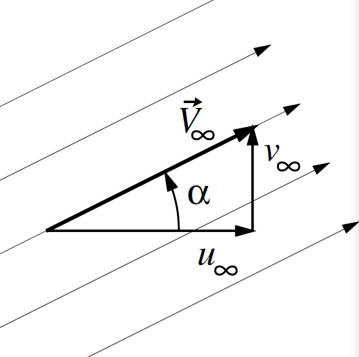
\includegraphics[width = 0.4\textwidth]{../img/diagram16.png}
\end{figure}
Cylindrical Coordinates:
\begin{gather}
  \phi (r, \theta) = V_{\infty} r \cos(\theta - \alpha)\\
  \psi (r, \theta) = V_{\infty} r \sin(\theta - \alpha)
\end{gather}
The conservation of mass is satisfied for cylindrical coordinates:
\begin{gather}
  \nabla \cdot \overrightarrow{V} = \frac{1}{r}\frac{\partial ru_r}{\partial r} + \frac{1}{r}\frac{\partial u_{\theta}}{\partial \theta} \\
  = \frac{\partial r(v_{\infty}\cos(\theta-\alpha))}{\partial r} - \frac{\partial v_{\infty}\sin(\theta-\alpha)}{\partial \theta} \\
  v_{\infty}\cos(\theta-\alpha) - v_{\infty}\cos(\theta-\alpha) = 0
\end{gather}
\begin{figure}[H]
  \centering
  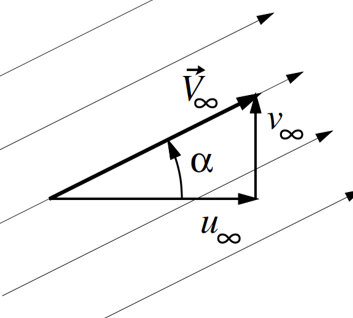
\includegraphics[width = 0.4\textwidth]{../img/diagram17.png}
\end{figure}
\section{Source/Sink Flow}
Cartesian Coordinates:
\begin{gather}
  \phi = \frac{\Lambda}{2\pi} \ln(\sqrt{x^2 +y^2})\\
  \psi = \frac{\Lambda}{2\pi}\arctan\left(\frac{y}{x}\right)
\end{gather}
Cylindrical Coordinates:
\begin{gather}
  \phi = \frac{\Lambda}{2\pi}\ln(r)\\
  \psi = \frac{\Lambda}{2\pi}\theta
\end{gather}
\begin{figure}[H]
  \centering
  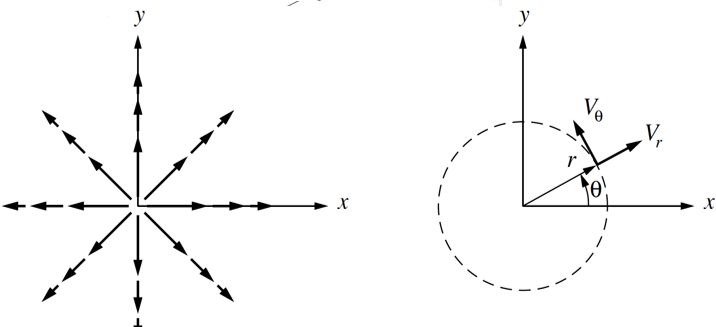
\includegraphics[width = 0.8\textwidth]{../img/diagram18.png}
\end{figure}
In cylindrical coordinates, we do not have a $\theta$ component as it is moving radially outwards from a source.
\begin{gather}
  u_r = \frac{\partial \phi}{\partial r} = \frac{\Lambda}{2\pi r}\\
  u_{\theta} = \frac{1}{r} \frac{\partial \phi}{\partial \theta} = 0
\end{gather}
Here we can see the magnitude of the velocity is dependent on $\frac{1}{r}$. If $\Lambda > 0$, we have a source and if $\Lambda < 0$, we have a sink.
\section{Uniform Flow + Source}
\begin{gather}
  \phi (r,\theta) = \frac{\Lambda}{2\pi} \ln(r) + V_{\infty} r \cos \theta \\
  \psi (r,\theta) = \frac{\Lambda}{2\pi}\theta + V_{\infty} r \sin \theta
\end{gather}
Stream function $\psi (r,\theta)$ of:
\begin{figure}[H]
  \centering
  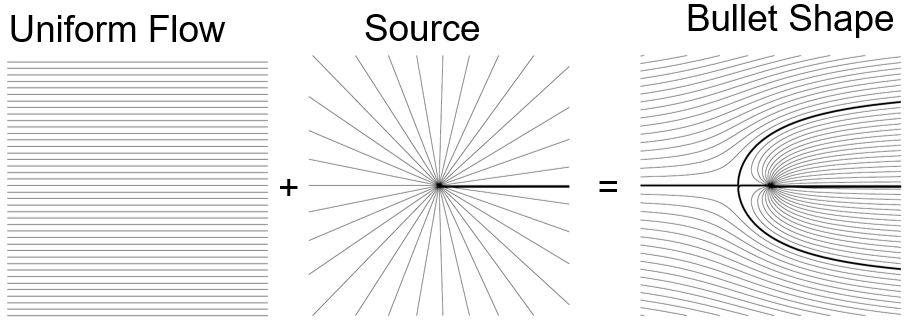
\includegraphics[width = 0.8\textwidth]{../img/diagram19.png}
\end{figure}
\section{Uniform Flow + Source + Sink}
\begin{gather}
  \phi - V_{\infty} r \cos \theta + \frac{\Lambda}{2\pi}(\ln (r_1) - \ln (r_2))\\
  \psi = V_{\infty} r \sin \theta + \frac{\Lambda}{2\pi} (\theta_1 - \theta_2)
\end{gather}
\begin{figure}[H]
  \centering
  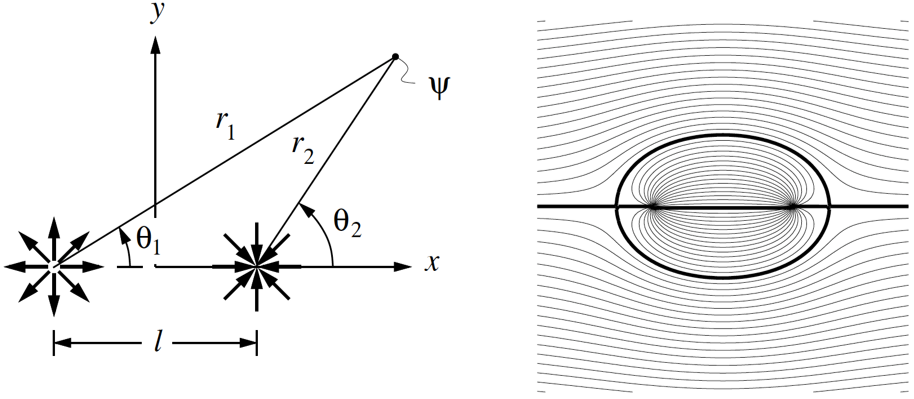
\includegraphics[width = 0.8\textwidth]{../img/diagram20.png}
\end{figure}
\section{Doublet}
Consider a pair of source and sink of $\pm \Lambda$ who are $l$ apart and $l\times\Lambda = $ constant.
\begin{gather}
  \psi =\lim_{l\rightarrow 0} \frac{\Lambda}{2\pi} (\theta_1 - \theta_2) = -\frac{k}{2\pi} \frac{\sin \theta}{r} \\
  \phi = \frac{k}{2\pi} \frac{\cos \theta}{r}
\end{gather}
\begin{figure}[H]
  \centering
  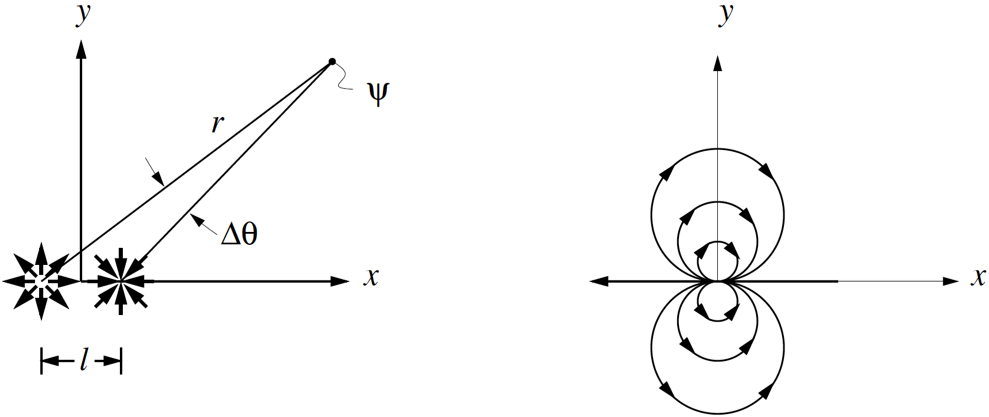
\includegraphics[width = 0.8\textwidth]{../img/diagram21.png}
\end{figure}
\section{Cylinder (Uniform Flow + Doublet)}
\begin{gather}
  \phi = V_{\infty}r\cos\theta + \frac{k}{2\pi} \frac{\cos\theta}{r}\\
  \psi = V_{\infty} r\sin\theta - \frac{k}{2\pi}\frac{\sin\theta}{r}
\end{gather}
\begin{figure}[H]
  \centering
  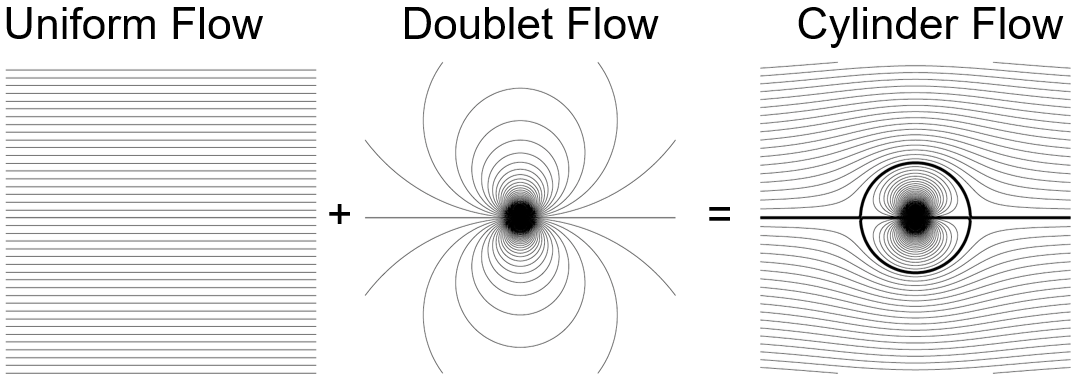
\includegraphics[width = 0.8\textwidth]{../img/diagram22.png}
\end{figure}
The radius of the cylinder can be derived as so:
\begin{gather}
  u_r = \frac{1}{r}\frac{\partial \psi}{\partial \theta} = V_{\infty} \cos\theta - \frac{k}{2\pi}\frac{\cos\theta}{r^2}\\
  u_{\theta} = -\frac{\partial \psi}{\partial r} = - \left( V_{\infty} \sin\theta + \frac{k}{2\pi}\frac{\sin\theta}{r^2} \right)
\end{gather}
On the cylinder, $\vec{u}\cdot\hat{n} = 0$
\begin{gather}
  \hat{n} = \hat{i}_r \rightarrow u_r(R)=0\\
  V_{\infty}\cos\theta - \frac{k}{2\pi}\frac{\cos\theta}{R^2} = 0\\
  R = \sqrt{\frac{k}{2\pi V_{\infty}}}
\end{gather}
We can rewrite $\phi$ and $\psi$
\begin{gather}
  \phi = V_{\infty}r\cos\theta\left(1+\frac{R^2}{r^2}\right)\\
  \psi = V_{\infty}r\sin\theta\left(1-\frac{R^2}{r^2}\right)
\end{gather}
On the cylinder surface, $r =R$ and inputting this into $\psi$:
\begin{equation}
  \psi = 0
\end{equation}
\section{Uniform Stream with Varying Direction}
All we need to do to generalise our equations a bit more is to rewrite our equations with an extra angular term, $\alpha$:
\begin{gather}
  \phi = V_{\infty}r\cos(\theta-\alpha)\left(1+\frac{R^2}{r^2}\right)\\
  \psi = V_{\infty}r\sin(\theta-\alpha)\left(1-\frac{R^2}{r^2}\right)
\end{gather}
\begin{figure}[H]
  \centering
  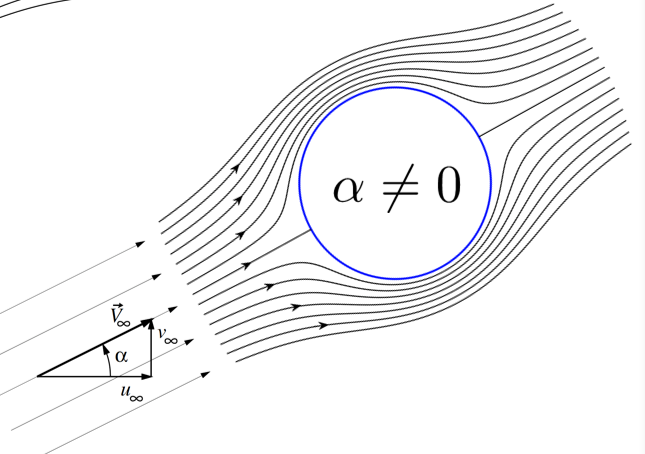
\includegraphics[width = 0.8\textwidth]{../img/diagram23.png}
\end{figure}
\section{Adding Circulation with a Vortex Flow}
\begin{gather}
  \phi = -\frac{\Gamma}{2\pi}\theta\\
  \psi = \frac{\Gamma}{2\pi}\ln\left(\frac{r}{R}\right)\\
  u_r = \frac{1}{r}\frac{\partial \psi}{\partial \theta} = 0\\
  u_{\theta} = -\frac{\partial \psi}{\partial r} = -\frac{\Gamma}{2\pi r}
\end{gather}
Where $\Gamma < 0$ is anti-clockwise motion and $\Gamma > 0$ is clockwise motion.
\begin{figure}[H]
  \centering
  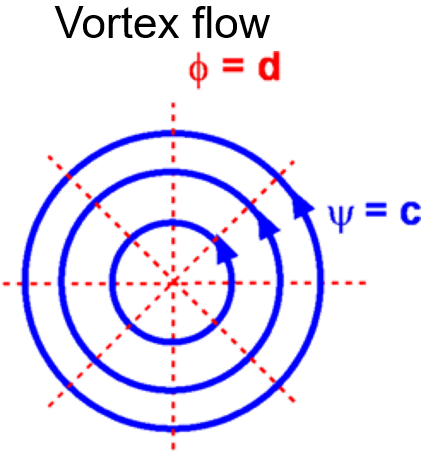
\includegraphics[width = 0.4\textwidth]{../img/diagram24.png}
\end{figure}
\section{Cylinder with a Vortex Flow}
\begin{gather}
  \psi = V_{\infty}r\sin\theta\left(1-\frac{R^2}{r^2}\right) + \frac{\Gamma}{2\pi}\ln\left(\frac{r}{R}\right)\\
  \phi = V_{\infty}r\cos\theta\left(1+\frac{R^2}{r^2}\right)-\frac{\Gamma}{2\pi}\theta\\
  u_r = \frac{1}{r}\frac{\partial \psi}{\partial \theta} = V_{\infty}\cos\theta\left(1-\frac{R^2}{r^2}\right)\\
  u_{\theta} = -\frac{\partial \psi}{\partial r} = - V_{\infty}\sin\theta\left(1+\frac{R^2}{r^2}\right)
\end{gather}
\begin{figure}[H]
  \centering
  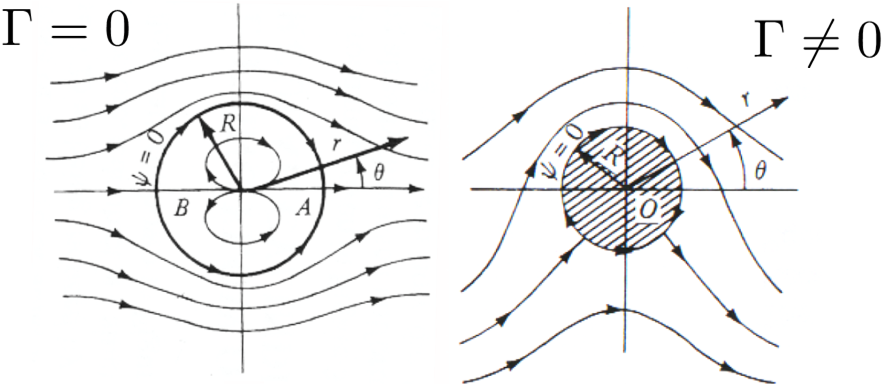
\includegraphics[width = 0.8\textwidth]{../img/diagram25.png}
\end{figure}
\section{Lift and Drag of a Cylinder with Circulation}
Apply Bernoulli:
\begin{gather}
  p_{\infty} + \frac{1}{2}\rho V_{\infty}^2 = p(r,\theta) + \frac{1}{2}\rho(u_r^2+u_{\theta}^2)\\
  c_p = \frac{p - p_{\infty}}{\frac{1}{2}\rho V_{\infty}^2} = 1 - \frac{u_r^2 + u_{\theta}^2}{V_{\infty}^2}
\end{gather}
On the cylinder surface: $u_r = 0$
\begin{gather}
  c_p (R,\theta) = 1 - \frac{u_{\theta}^2}{V_{\infty}^2}=1-\frac{(2V_{\infty}\sin\theta + \frac{\Gamma}{2\pi R})^2}{V_{\infty}^2} \\
  = 1-\left(4\sin^2(\theta)+\frac{\Gamma^2}{4\pi^2V_{\infty}^2R^2}+\frac{2\Gamma\sin(\theta)}{V_{\infty}\pi R}\right)
\end{gather}
\section{Lift of the Cylinder}
We need to calculate $c_p$ on the surface of the cylinder.
\begin{align}
  L &= -\frac{1}{2}\rho V_{\infty}^2\int_{0}^{2\pi} \left(c_p \cdot \hat{n}\cdot\hat{j}R\right)\dif \theta \\
  &= - \frac{1}{2}\rho V_{\infty}^2 \int_{0}^{2\pi} \left(c_p \sin\theta R\right) \,\mathrm{d}\theta \\
  L &= -\frac{1}{2}\rho V_{\infty}^2 \int_{0}^{2\pi} \left(1-\frac{(2V_{\infty}\sin\theta + \frac{\Gamma}{2\pi R})^2}{V_{\infty}^2}\right) \sin\theta R \,\mathrm{d}\theta 
\end{align}
\end{document}